\documentclass[twoside]{book}

% Packages required by doxygen
\usepackage{fixltx2e}
\usepackage{calc}
\usepackage{doxygen}
\usepackage[export]{adjustbox} % also loads graphicx
\usepackage{graphicx}
\usepackage[utf8]{inputenc}
\usepackage{makeidx}
\usepackage{multicol}
\usepackage{multirow}
\PassOptionsToPackage{warn}{textcomp}
\usepackage{textcomp}
\usepackage[nointegrals]{wasysym}
\usepackage[table]{xcolor}

% Font selection
\usepackage[T1]{fontenc}
\usepackage[scaled=.90]{helvet}
\usepackage{courier}
\usepackage{amssymb}
\usepackage{sectsty}
\renewcommand{\familydefault}{\sfdefault}
\allsectionsfont{%
  \fontseries{bc}\selectfont%
  \color{darkgray}%
}
\renewcommand{\DoxyLabelFont}{%
  \fontseries{bc}\selectfont%
  \color{darkgray}%
}
\newcommand{\+}{\discretionary{\mbox{\scriptsize$\hookleftarrow$}}{}{}}

% Page & text layout
\usepackage{geometry}
\geometry{%
  a4paper,%
  top=2.5cm,%
  bottom=2.5cm,%
  left=2.5cm,%
  right=2.5cm%
}
\tolerance=750
\hfuzz=15pt
\hbadness=750
\setlength{\emergencystretch}{15pt}
\setlength{\parindent}{0cm}
\setlength{\parskip}{3ex plus 2ex minus 2ex}
\makeatletter
\renewcommand{\paragraph}{%
  \@startsection{paragraph}{4}{0ex}{-1.0ex}{1.0ex}{%
    \normalfont\normalsize\bfseries\SS@parafont%
  }%
}
\renewcommand{\subparagraph}{%
  \@startsection{subparagraph}{5}{0ex}{-1.0ex}{1.0ex}{%
    \normalfont\normalsize\bfseries\SS@subparafont%
  }%
}
\makeatother

% Headers & footers
\usepackage{fancyhdr}
\pagestyle{fancyplain}
\fancyhead[LE]{\fancyplain{}{\bfseries\thepage}}
\fancyhead[CE]{\fancyplain{}{}}
\fancyhead[RE]{\fancyplain{}{\bfseries\leftmark}}
\fancyhead[LO]{\fancyplain{}{\bfseries\rightmark}}
\fancyhead[CO]{\fancyplain{}{}}
\fancyhead[RO]{\fancyplain{}{\bfseries\thepage}}
\fancyfoot[LE]{\fancyplain{}{}}
\fancyfoot[CE]{\fancyplain{}{}}
\fancyfoot[RE]{\fancyplain{}{\bfseries\scriptsize Generated by Doxygen }}
\fancyfoot[LO]{\fancyplain{}{\bfseries\scriptsize Generated by Doxygen }}
\fancyfoot[CO]{\fancyplain{}{}}
\fancyfoot[RO]{\fancyplain{}{}}
\renewcommand{\footrulewidth}{0.4pt}
\renewcommand{\chaptermark}[1]{%
  \markboth{#1}{}%
}
\renewcommand{\sectionmark}[1]{%
  \markright{\thesection\ #1}%
}

% Indices & bibliography
\usepackage{natbib}
\usepackage[titles]{tocloft}
\setcounter{tocdepth}{3}
\setcounter{secnumdepth}{5}
\makeindex

% Hyperlinks (required, but should be loaded last)
\usepackage{ifpdf}
\ifpdf
  \usepackage[pdftex,pagebackref=true]{hyperref}
\else
  \usepackage[ps2pdf,pagebackref=true]{hyperref}
\fi
\hypersetup{%
  colorlinks=true,%
  linkcolor=blue,%
  citecolor=blue,%
  unicode%
}

% Custom commands
\newcommand{\clearemptydoublepage}{%
  \newpage{\pagestyle{empty}\cleardoublepage}%
}

\usepackage{caption}
\captionsetup{labelsep=space,justification=centering,font={bf},singlelinecheck=off,skip=4pt,position=top}

%===== C O N T E N T S =====

\begin{document}

% Titlepage & ToC
\hypersetup{pageanchor=false,
             bookmarksnumbered=true,
             pdfencoding=unicode
            }
\pagenumbering{alph}
\begin{titlepage}
\vspace*{7cm}
\begin{center}%
{\Large Inter-\/\+Process Communication For Order \\[1ex]\large 1.\+0 }\\
\vspace*{1cm}
{\large Generated by Doxygen 1.8.13}\\
\end{center}
\end{titlepage}
\clearemptydoublepage
\pagenumbering{roman}
\tableofcontents
\clearemptydoublepage
\pagenumbering{arabic}
\hypersetup{pageanchor=true}

%--- Begin generated contents ---
\chapter{Namespace Index}
\section{Namespace List}
Here is a list of all namespaces with brief descriptions\+:\begin{DoxyCompactList}
\item\contentsline{section}{\hyperlink{namespaceinterprocess}{interprocess} }{\pageref{namespaceinterprocess}}{}
\end{DoxyCompactList}

\chapter{Hierarchical Index}
\section{Class Hierarchy}
This inheritance list is sorted roughly, but not completely, alphabetically\+:\begin{DoxyCompactList}
\item \contentsline{section}{interprocess.\+Interprocess}{\pageref{classinterprocess_1_1_interprocess}}{}
\item \contentsline{section}{interprocess.\+Json\+Parser}{\pageref{classinterprocess_1_1_json_parser}}{}
\item \contentsline{section}{interprocess.\+Order}{\pageref{classinterprocess_1_1_order}}{}
\item Thread\begin{DoxyCompactList}
\item \contentsline{section}{interprocess.\+Message}{\pageref{classinterprocess_1_1_message}}{}
\end{DoxyCompactList}
\end{DoxyCompactList}

\chapter{Class Index}
\section{Class List}
Here are the classes, structs, unions and interfaces with brief descriptions\+:\begin{DoxyCompactList}
\item\contentsline{section}{\hyperlink{classinterprocess_1_1_interprocess}{interprocess.\+Interprocess} }{\pageref{classinterprocess_1_1_interprocess}}{}
\item\contentsline{section}{\hyperlink{classinterprocess_1_1_json_parser}{interprocess.\+Json\+Parser} }{\pageref{classinterprocess_1_1_json_parser}}{}
\item\contentsline{section}{\hyperlink{classinterprocess_1_1_message}{interprocess.\+Message} }{\pageref{classinterprocess_1_1_message}}{}
\item\contentsline{section}{\hyperlink{classinterprocess_1_1_order}{interprocess.\+Order} }{\pageref{classinterprocess_1_1_order}}{}
\end{DoxyCompactList}

\chapter{File Index}
\section{File List}
Here is a list of all files with brief descriptions\+:\begin{DoxyCompactList}
\item\contentsline{section}{src/interprocess/\hyperlink{_interprocess_8java}{Interprocess.\+java} }{\pageref{_interprocess_8java}}{}
\item\contentsline{section}{src/interprocess/\hyperlink{_json_parser_8java}{Json\+Parser.\+java} }{\pageref{_json_parser_8java}}{}
\item\contentsline{section}{src/interprocess/\hyperlink{_message_8java}{Message.\+java} }{\pageref{_message_8java}}{}
\item\contentsline{section}{src/interprocess/\hyperlink{_order_8java}{Order.\+java} }{\pageref{_order_8java}}{}
\end{DoxyCompactList}

\chapter{Namespace Documentation}
\hypertarget{namespaceinterprocess}{}\section{Package interprocess}
\label{namespaceinterprocess}\index{interprocess@{interprocess}}
\subsection*{Classes}
\begin{DoxyCompactItemize}
\item 
class \hyperlink{classinterprocess_1_1_interprocess}{Interprocess}
\item 
class \hyperlink{classinterprocess_1_1_json_parser}{Json\+Parser}
\item 
class \hyperlink{classinterprocess_1_1_message}{Message}
\item 
class \hyperlink{classinterprocess_1_1_order}{Order}
\end{DoxyCompactItemize}

\chapter{Class Documentation}
\hypertarget{classinterprocess_1_1_interprocess}{}\section{interprocess.\+Interprocess Class Reference}
\label{classinterprocess_1_1_interprocess}\index{interprocess.\+Interprocess@{interprocess.\+Interprocess}}
\subsection*{Static Public Member Functions}
\begin{DoxyCompactItemize}
\item 
static void \hyperlink{classinterprocess_1_1_interprocess_a62de3e766ef3c3c70e60feda45bd3557}{main} (String\mbox{[}$\,$\mbox{]} args)  throws I\+O\+Exception, Interrupted\+Exception      
\end{DoxyCompactItemize}


\subsection{Detailed Description}
\hyperlink{classinterprocess_1_1_interprocess}{Interprocess} --- This main class contains thread to run the pipes method. 

This is a multi-\/threaded communication.

This will focus on part of the process since one process has many threads. \begin{DoxyAuthor}{Author}
Van Do 
\end{DoxyAuthor}
\begin{DoxyVersion}{Version}
1.\+0 
\end{DoxyVersion}


\subsection{Member Function Documentation}
\mbox{\Hypertarget{classinterprocess_1_1_interprocess_a62de3e766ef3c3c70e60feda45bd3557}\label{classinterprocess_1_1_interprocess_a62de3e766ef3c3c70e60feda45bd3557}} 
\index{interprocess\+::\+Interprocess@{interprocess\+::\+Interprocess}!main@{main}}
\index{main@{main}!interprocess\+::\+Interprocess@{interprocess\+::\+Interprocess}}
\subsubsection{\texorpdfstring{main()}{main()}}
{\footnotesize\ttfamily static void interprocess.\+Interprocess.\+main (\begin{DoxyParamCaption}\item[{String \mbox{[}$\,$\mbox{]}}]{args }\end{DoxyParamCaption}) throws I\+O\+Exception, Interrupted\+Exception\hspace{0.3cm}{\ttfamily [inline]}, {\ttfamily [static]}}

This static void contains the runnable program for connect an inter-\/process communication using pipes. 
\begin{DoxyParams}{Parameters}
{\em args} & -\/ the command line arguments. \\
\hline
\end{DoxyParams}

\begin{DoxyExceptions}{Exceptions}
{\em I\+O\+Exception} & -\/ if input is does not meet with the variables. \\
\hline
{\em Interrupted\+Exception} & -\/ if pipe is interrupted, it cannot complete the action of sending and receiving. \\
\hline
\end{DoxyExceptions}


The documentation for this class was generated from the following file\+:\begin{DoxyCompactItemize}
\item 
src/interprocess/\hyperlink{_interprocess_8java}{Interprocess.\+java}\end{DoxyCompactItemize}

\hypertarget{classinterprocess_1_1_json_parser}{}\section{interprocess.\+Json\+Parser Class Reference}
\label{classinterprocess_1_1_json_parser}\index{interprocess.\+Json\+Parser@{interprocess.\+Json\+Parser}}
\subsection*{Public Member Functions}
\begin{DoxyCompactItemize}
\item 
String \hyperlink{classinterprocess_1_1_json_parser_a71acd9266626b51692367dcadab6bdb3}{serialize\+Colours} (List$<$ \hyperlink{classinterprocess_1_1_order}{Order} $>$ list)
\item 
List$<$ \hyperlink{classinterprocess_1_1_order}{Order} $>$ \hyperlink{classinterprocess_1_1_json_parser_aedad98ba21bcb5476a00ac4c66267c57}{deserialize\+Colours} (String input\+Json\+String)
\end{DoxyCompactItemize}


\subsection{Detailed Description}
\hyperlink{classinterprocess_1_1_json_parser}{Json\+Parser} --- This class contains method to translate list of \hyperlink{classinterprocess_1_1_order}{Order} objects to J\+S\+ON string and back. \begin{DoxyAuthor}{Author}
Van Do 
\end{DoxyAuthor}


\subsection{Member Function Documentation}
\mbox{\Hypertarget{classinterprocess_1_1_json_parser_aedad98ba21bcb5476a00ac4c66267c57}\label{classinterprocess_1_1_json_parser_aedad98ba21bcb5476a00ac4c66267c57}} 
\index{interprocess\+::\+Json\+Parser@{interprocess\+::\+Json\+Parser}!deserialize\+Colours@{deserialize\+Colours}}
\index{deserialize\+Colours@{deserialize\+Colours}!interprocess\+::\+Json\+Parser@{interprocess\+::\+Json\+Parser}}
\subsubsection{\texorpdfstring{deserialize\+Colours()}{deserializeColours()}}
{\footnotesize\ttfamily List$<$\hyperlink{classinterprocess_1_1_order}{Order}$>$ interprocess.\+Json\+Parser.\+deserialize\+Colours (\begin{DoxyParamCaption}\item[{String}]{input\+Json\+String }\end{DoxyParamCaption})\hspace{0.3cm}{\ttfamily [inline]}}

Translate J\+S\+ON string to list of \hyperlink{classinterprocess_1_1_order}{Order} objects. 
\begin{DoxyParams}{Parameters}
{\em input\+Json\+String} & -\/ the J\+S\+ON string contains \hyperlink{classinterprocess_1_1_order}{Order} objects and will convert to list. \\
\hline
\end{DoxyParams}
\begin{DoxyReturn}{Returns}
the list of \hyperlink{classinterprocess_1_1_order}{Order} objects. 
\end{DoxyReturn}
\mbox{\Hypertarget{classinterprocess_1_1_json_parser_a71acd9266626b51692367dcadab6bdb3}\label{classinterprocess_1_1_json_parser_a71acd9266626b51692367dcadab6bdb3}} 
\index{interprocess\+::\+Json\+Parser@{interprocess\+::\+Json\+Parser}!serialize\+Colours@{serialize\+Colours}}
\index{serialize\+Colours@{serialize\+Colours}!interprocess\+::\+Json\+Parser@{interprocess\+::\+Json\+Parser}}
\subsubsection{\texorpdfstring{serialize\+Colours()}{serializeColours()}}
{\footnotesize\ttfamily String interprocess.\+Json\+Parser.\+serialize\+Colours (\begin{DoxyParamCaption}\item[{List$<$ \hyperlink{classinterprocess_1_1_order}{Order} $>$}]{list }\end{DoxyParamCaption})\hspace{0.3cm}{\ttfamily [inline]}}

Serialize a list of order into J\+S\+ON string. 
\begin{DoxyParams}{Parameters}
{\em list} & -\/ a list of \hyperlink{classinterprocess_1_1_order}{Order} objects from the user input. \\
\hline
\end{DoxyParams}
\begin{DoxyReturn}{Returns}
J\+S\+ON string that was being translate from list. 
\end{DoxyReturn}


The documentation for this class was generated from the following file\+:\begin{DoxyCompactItemize}
\item 
src/interprocess/\hyperlink{_json_parser_8java}{Json\+Parser.\+java}\end{DoxyCompactItemize}

\hypertarget{classinterprocess_1_1_message}{}\section{interprocess.\+Message Class Reference}
\label{classinterprocess_1_1_message}\index{interprocess.\+Message@{interprocess.\+Message}}
Inheritance diagram for interprocess.\+Message\+:\begin{figure}[H]
\begin{center}
\leavevmode
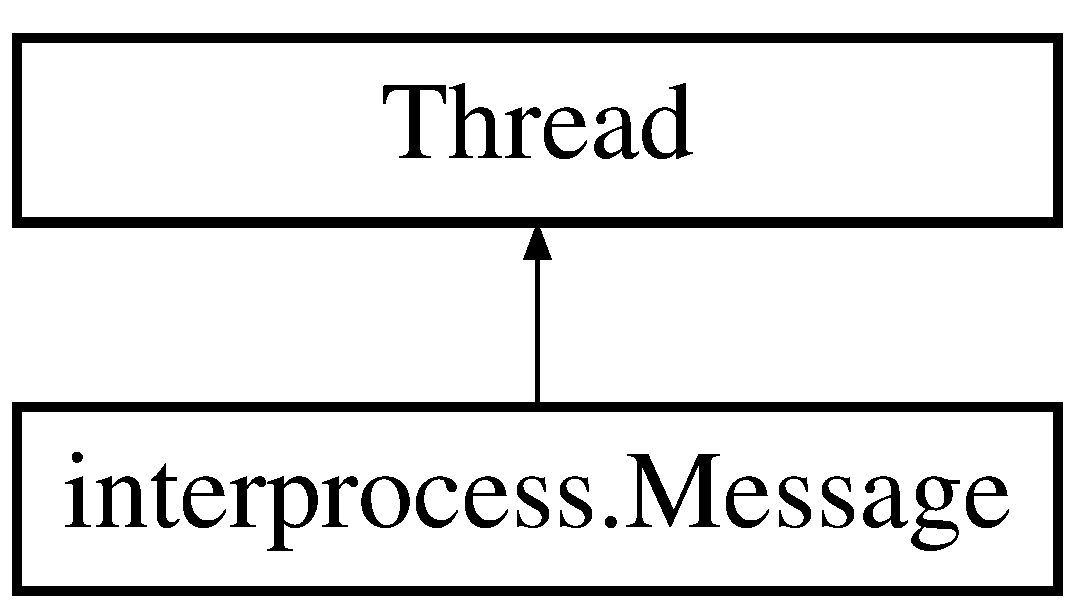
\includegraphics[height=2.000000cm]{classinterprocess_1_1_message}
\end{center}
\end{figure}
\subsection*{Public Member Functions}
\begin{DoxyCompactItemize}
\item 
void \hyperlink{classinterprocess_1_1_message_a753fc2d9bffff59d32d9a20512ac6639}{produce\+Order} (Piped\+Output\+Stream output, List$<$ \hyperlink{classinterprocess_1_1_order}{Order} $>$ order)
\item 
void \hyperlink{classinterprocess_1_1_message_ada4c768cf0688deaede00d43220fd100}{consume\+Order} (Piped\+Input\+Stream input)
\item 
void \hyperlink{classinterprocess_1_1_message_a66e94ca490a4bae0e26db95052aa3956}{add\+Order} (Piped\+Output\+Stream output)
\end{DoxyCompactItemize}
\subsection*{Private Member Functions}
\begin{DoxyCompactItemize}
\item 
int \hyperlink{classinterprocess_1_1_message_a594aec63ced8dc0b7440ceae46e71c52}{handle\+Int} ()
\item 
boolean \hyperlink{classinterprocess_1_1_message_a67f6da8b5552745401b1ab20f3f8a035}{is\+String\+Null\+Or\+White\+Space} (String value)
\end{DoxyCompactItemize}


\subsection{Detailed Description}
\hyperlink{classinterprocess_1_1_message}{Message} --- This class allows to read or write message stream from one end of the pipe to another end. \begin{DoxyAuthor}{Author}
Van Do 
\end{DoxyAuthor}


\subsection{Member Function Documentation}
\mbox{\Hypertarget{classinterprocess_1_1_message_a66e94ca490a4bae0e26db95052aa3956}\label{classinterprocess_1_1_message_a66e94ca490a4bae0e26db95052aa3956}} 
\index{interprocess\+::\+Message@{interprocess\+::\+Message}!add\+Order@{add\+Order}}
\index{add\+Order@{add\+Order}!interprocess\+::\+Message@{interprocess\+::\+Message}}
\subsubsection{\texorpdfstring{add\+Order()}{addOrder()}}
{\footnotesize\ttfamily void interprocess.\+Message.\+add\+Order (\begin{DoxyParamCaption}\item[{Piped\+Output\+Stream}]{output }\end{DoxyParamCaption})\hspace{0.3cm}{\ttfamily [inline]}}

Create a list of orders by user interface. 
\begin{DoxyParams}{Parameters}
{\em output} & using output piped stream for produce order method to enable to connect pipes. \\
\hline
\end{DoxyParams}
\mbox{\Hypertarget{classinterprocess_1_1_message_ada4c768cf0688deaede00d43220fd100}\label{classinterprocess_1_1_message_ada4c768cf0688deaede00d43220fd100}} 
\index{interprocess\+::\+Message@{interprocess\+::\+Message}!consume\+Order@{consume\+Order}}
\index{consume\+Order@{consume\+Order}!interprocess\+::\+Message@{interprocess\+::\+Message}}
\subsubsection{\texorpdfstring{consume\+Order()}{consumeOrder()}}
{\footnotesize\ttfamily void interprocess.\+Message.\+consume\+Order (\begin{DoxyParamCaption}\item[{Piped\+Input\+Stream}]{input }\end{DoxyParamCaption})\hspace{0.3cm}{\ttfamily [inline]}}

Read J\+S\+ON string from piped output stream and convert into list of \hyperlink{classinterprocess_1_1_order}{Order} objects to make it readable for the receiver. 
\begin{DoxyParams}{Parameters}
{\em input} & convert byte of data from piped output stream and convert into array of characters. \\
\hline
\end{DoxyParams}

\begin{DoxyExceptions}{Exceptions}
{\em I\+O\+Exception} & -\/ catch errors when stream of bytes was unable to be read. \\
\hline
\end{DoxyExceptions}
\mbox{\Hypertarget{classinterprocess_1_1_message_a594aec63ced8dc0b7440ceae46e71c52}\label{classinterprocess_1_1_message_a594aec63ced8dc0b7440ceae46e71c52}} 
\index{interprocess\+::\+Message@{interprocess\+::\+Message}!handle\+Int@{handle\+Int}}
\index{handle\+Int@{handle\+Int}!interprocess\+::\+Message@{interprocess\+::\+Message}}
\subsubsection{\texorpdfstring{handle\+Int()}{handleInt()}}
{\footnotesize\ttfamily int interprocess.\+Message.\+handle\+Int (\begin{DoxyParamCaption}{ }\end{DoxyParamCaption})\hspace{0.3cm}{\ttfamily [inline]}, {\ttfamily [private]}}

Handling integer input. 
\begin{DoxyExceptions}{Exceptions}
{\em Input\+Mismatch\+Exception} & -\/ catch if input does not match integer requirement. \\
\hline
\end{DoxyExceptions}
\begin{DoxyReturn}{Returns}
integer value 
\end{DoxyReturn}
\mbox{\Hypertarget{classinterprocess_1_1_message_a67f6da8b5552745401b1ab20f3f8a035}\label{classinterprocess_1_1_message_a67f6da8b5552745401b1ab20f3f8a035}} 
\index{interprocess\+::\+Message@{interprocess\+::\+Message}!is\+String\+Null\+Or\+White\+Space@{is\+String\+Null\+Or\+White\+Space}}
\index{is\+String\+Null\+Or\+White\+Space@{is\+String\+Null\+Or\+White\+Space}!interprocess\+::\+Message@{interprocess\+::\+Message}}
\subsubsection{\texorpdfstring{is\+String\+Null\+Or\+White\+Space()}{isStringNullOrWhiteSpace()}}
{\footnotesize\ttfamily boolean interprocess.\+Message.\+is\+String\+Null\+Or\+White\+Space (\begin{DoxyParamCaption}\item[{String}]{value }\end{DoxyParamCaption})\hspace{0.3cm}{\ttfamily [inline]}, {\ttfamily [private]}}

Handling string input for emptiness. 
\begin{DoxyParams}{Parameters}
{\em value} & the string input by the user. \\
\hline
\end{DoxyParams}
\begin{DoxyReturn}{Returns}
the statement of the string is not empty. 
\end{DoxyReturn}
\mbox{\Hypertarget{classinterprocess_1_1_message_a753fc2d9bffff59d32d9a20512ac6639}\label{classinterprocess_1_1_message_a753fc2d9bffff59d32d9a20512ac6639}} 
\index{interprocess\+::\+Message@{interprocess\+::\+Message}!produce\+Order@{produce\+Order}}
\index{produce\+Order@{produce\+Order}!interprocess\+::\+Message@{interprocess\+::\+Message}}
\subsubsection{\texorpdfstring{produce\+Order()}{produceOrder()}}
{\footnotesize\ttfamily void interprocess.\+Message.\+produce\+Order (\begin{DoxyParamCaption}\item[{Piped\+Output\+Stream}]{output,  }\item[{List$<$ \hyperlink{classinterprocess_1_1_order}{Order} $>$}]{order }\end{DoxyParamCaption})\hspace{0.3cm}{\ttfamily [inline]}}

Convert the list of \hyperlink{classinterprocess_1_1_order}{Order} objects into J\+S\+ON string. Write the J\+S\+ON string into bytes and send to Piped\+Input\+Stream. See \hyperlink{classinterprocess_1_1_message_ada4c768cf0688deaede00d43220fd100}{consume\+Order}. 
\begin{DoxyParams}{Parameters}
{\em output} & connected to piped input stream where this pipe writes J\+S\+ON string in bytes to receiver. \\
\hline
{\em order} & list of \hyperlink{classinterprocess_1_1_order}{Order} objects by user. \\
\hline
\end{DoxyParams}

\begin{DoxyExceptions}{Exceptions}
{\em Unsupported\+Encoding\+Exception} & -\/ catch errors when the message encoding into bytes have failed. \\
\hline
{\em I\+O\+Exception} & -\/ catch errors if write stream of bytes to pipe output stream has failed. \\
\hline
\end{DoxyExceptions}


The documentation for this class was generated from the following file\+:\begin{DoxyCompactItemize}
\item 
src/interprocess/\hyperlink{_message_8java}{Message.\+java}\end{DoxyCompactItemize}

\hypertarget{classinterprocess_1_1_order}{}\section{interprocess.\+Order Class Reference}
\label{classinterprocess_1_1_order}\index{interprocess.\+Order@{interprocess.\+Order}}
\subsection*{Public Member Functions}
\begin{DoxyCompactItemize}
\item 
\hyperlink{classinterprocess_1_1_order_a5e5c6892a7af1a49723b0d5c5406bdd6}{Order} ()
\item 
\hyperlink{classinterprocess_1_1_order_af13a7737eb33a202266166c9c1a59227}{Order} (String product, int quantity, String customer, String address)
\item 
String \hyperlink{classinterprocess_1_1_order_a06e815c40a345dcedbed2765784de66b}{get\+Product} ()
\item 
int \hyperlink{classinterprocess_1_1_order_ad38dbbe0a5126da82d8078b8b3295ce9}{get\+Quantity} ()
\item 
String \hyperlink{classinterprocess_1_1_order_a052b610505ed3911bfd95da17d94aaf9}{get\+Name} ()
\item 
String \hyperlink{classinterprocess_1_1_order_a90730d59b1d16c809a8a5c504c735170}{get\+Address} ()
\item 
void \hyperlink{classinterprocess_1_1_order_a2c98ed99009d1303270a768bb3fdd4f4}{set\+Product} (String name)
\item 
void \hyperlink{classinterprocess_1_1_order_ae25cc04154fec8d5025154eca104f752}{set\+Quantity} (int quantity)
\item 
void \hyperlink{classinterprocess_1_1_order_a175bac96d567d6fe6cc7829275f58451}{set\+Name} (String name)
\item 
void \hyperlink{classinterprocess_1_1_order_a0264f8cb97eb1a9e0bc445b2ea3a6b55}{set\+Address} (String address)
\item 
void \hyperlink{classinterprocess_1_1_order_a780af8945598d5b31d124e0309c4ae65}{print\+Details} ()
\end{DoxyCompactItemize}
\subsection*{Private Attributes}
\begin{DoxyCompactItemize}
\item 
String \hyperlink{classinterprocess_1_1_order_ab22f659fd57c8bde1b362e7054d63f61}{product\+Name}
\item 
int \hyperlink{classinterprocess_1_1_order_a471467d213a750ba99fc21e9d468fe98}{product\+Quantity}
\item 
String \hyperlink{classinterprocess_1_1_order_a15fc1e10e5935f82493a68ebd9ef1a55}{customer\+Name}
\item 
String \hyperlink{classinterprocess_1_1_order_a681c40b962e58237454c9feaae2610d9}{customer\+Address}
\end{DoxyCompactItemize}


\subsection{Detailed Description}
\hyperlink{classinterprocess_1_1_order}{Order} --- This class contains data of order. \begin{DoxyAuthor}{Author}
Van Do 
\end{DoxyAuthor}


\subsection{Constructor \& Destructor Documentation}
\mbox{\Hypertarget{classinterprocess_1_1_order_a5e5c6892a7af1a49723b0d5c5406bdd6}\label{classinterprocess_1_1_order_a5e5c6892a7af1a49723b0d5c5406bdd6}} 
\index{interprocess\+::\+Order@{interprocess\+::\+Order}!Order@{Order}}
\index{Order@{Order}!interprocess\+::\+Order@{interprocess\+::\+Order}}
\subsubsection{\texorpdfstring{Order()}{Order()}\hspace{0.1cm}{\footnotesize\ttfamily [1/2]}}
{\footnotesize\ttfamily interprocess.\+Order.\+Order (\begin{DoxyParamCaption}{ }\end{DoxyParamCaption})\hspace{0.3cm}{\ttfamily [inline]}}

Null class constructor to access methods. \mbox{\Hypertarget{classinterprocess_1_1_order_af13a7737eb33a202266166c9c1a59227}\label{classinterprocess_1_1_order_af13a7737eb33a202266166c9c1a59227}} 
\index{interprocess\+::\+Order@{interprocess\+::\+Order}!Order@{Order}}
\index{Order@{Order}!interprocess\+::\+Order@{interprocess\+::\+Order}}
\subsubsection{\texorpdfstring{Order()}{Order()}\hspace{0.1cm}{\footnotesize\ttfamily [2/2]}}
{\footnotesize\ttfamily interprocess.\+Order.\+Order (\begin{DoxyParamCaption}\item[{String}]{product,  }\item[{int}]{quantity,  }\item[{String}]{customer,  }\item[{String}]{address }\end{DoxyParamCaption})\hspace{0.3cm}{\ttfamily [inline]}}

Parameterized constructor to store object\textquotesingle{}s order data. 
\begin{DoxyParams}{Parameters}
{\em product} & -\/ the name of the product. See \hyperlink{classinterprocess_1_1_order_ab22f659fd57c8bde1b362e7054d63f61}{product\+Name}. \\
\hline
{\em quantity} & -\/ the number of products. See \hyperlink{classinterprocess_1_1_order_a471467d213a750ba99fc21e9d468fe98}{product\+Quantity}. \\
\hline
{\em customer} & -\/ the customer\textquotesingle{}s name. See \hyperlink{classinterprocess_1_1_order_a15fc1e10e5935f82493a68ebd9ef1a55}{customer\+Name}. \\
\hline
{\em address} & -\/ the customer\textquotesingle{}s email or home address. See \hyperlink{classinterprocess_1_1_order_a681c40b962e58237454c9feaae2610d9}{customer\+Address}. \\
\hline
\end{DoxyParams}


\subsection{Member Function Documentation}
\mbox{\Hypertarget{classinterprocess_1_1_order_a90730d59b1d16c809a8a5c504c735170}\label{classinterprocess_1_1_order_a90730d59b1d16c809a8a5c504c735170}} 
\index{interprocess\+::\+Order@{interprocess\+::\+Order}!get\+Address@{get\+Address}}
\index{get\+Address@{get\+Address}!interprocess\+::\+Order@{interprocess\+::\+Order}}
\subsubsection{\texorpdfstring{get\+Address()}{getAddress()}}
{\footnotesize\ttfamily String interprocess.\+Order.\+get\+Address (\begin{DoxyParamCaption}{ }\end{DoxyParamCaption})\hspace{0.3cm}{\ttfamily [inline]}}

Get the customer\textquotesingle{}s address. See \hyperlink{classinterprocess_1_1_order_a681c40b962e58237454c9feaae2610d9}{customer\+Address}. \begin{DoxyReturn}{Returns}
customer\textquotesingle{}s address. 
\end{DoxyReturn}
\mbox{\Hypertarget{classinterprocess_1_1_order_a052b610505ed3911bfd95da17d94aaf9}\label{classinterprocess_1_1_order_a052b610505ed3911bfd95da17d94aaf9}} 
\index{interprocess\+::\+Order@{interprocess\+::\+Order}!get\+Name@{get\+Name}}
\index{get\+Name@{get\+Name}!interprocess\+::\+Order@{interprocess\+::\+Order}}
\subsubsection{\texorpdfstring{get\+Name()}{getName()}}
{\footnotesize\ttfamily String interprocess.\+Order.\+get\+Name (\begin{DoxyParamCaption}{ }\end{DoxyParamCaption})\hspace{0.3cm}{\ttfamily [inline]}}

Get the customer\textquotesingle{}s name. See \hyperlink{classinterprocess_1_1_order_a15fc1e10e5935f82493a68ebd9ef1a55}{customer\+Name}. \begin{DoxyReturn}{Returns}
customer\textquotesingle{}s name. 
\end{DoxyReturn}
\mbox{\Hypertarget{classinterprocess_1_1_order_a06e815c40a345dcedbed2765784de66b}\label{classinterprocess_1_1_order_a06e815c40a345dcedbed2765784de66b}} 
\index{interprocess\+::\+Order@{interprocess\+::\+Order}!get\+Product@{get\+Product}}
\index{get\+Product@{get\+Product}!interprocess\+::\+Order@{interprocess\+::\+Order}}
\subsubsection{\texorpdfstring{get\+Product()}{getProduct()}}
{\footnotesize\ttfamily String interprocess.\+Order.\+get\+Product (\begin{DoxyParamCaption}{ }\end{DoxyParamCaption})\hspace{0.3cm}{\ttfamily [inline]}}

Get the name of the product. See \hyperlink{classinterprocess_1_1_order_ab22f659fd57c8bde1b362e7054d63f61}{product\+Name}. \begin{DoxyReturn}{Returns}
name of the product. 
\end{DoxyReturn}
\mbox{\Hypertarget{classinterprocess_1_1_order_ad38dbbe0a5126da82d8078b8b3295ce9}\label{classinterprocess_1_1_order_ad38dbbe0a5126da82d8078b8b3295ce9}} 
\index{interprocess\+::\+Order@{interprocess\+::\+Order}!get\+Quantity@{get\+Quantity}}
\index{get\+Quantity@{get\+Quantity}!interprocess\+::\+Order@{interprocess\+::\+Order}}
\subsubsection{\texorpdfstring{get\+Quantity()}{getQuantity()}}
{\footnotesize\ttfamily int interprocess.\+Order.\+get\+Quantity (\begin{DoxyParamCaption}{ }\end{DoxyParamCaption})\hspace{0.3cm}{\ttfamily [inline]}}

Get the number of products. See \hyperlink{classinterprocess_1_1_order_a471467d213a750ba99fc21e9d468fe98}{product\+Quantity}. \begin{DoxyReturn}{Returns}
number of products. 
\end{DoxyReturn}
\mbox{\Hypertarget{classinterprocess_1_1_order_a780af8945598d5b31d124e0309c4ae65}\label{classinterprocess_1_1_order_a780af8945598d5b31d124e0309c4ae65}} 
\index{interprocess\+::\+Order@{interprocess\+::\+Order}!print\+Details@{print\+Details}}
\index{print\+Details@{print\+Details}!interprocess\+::\+Order@{interprocess\+::\+Order}}
\subsubsection{\texorpdfstring{print\+Details()}{printDetails()}}
{\footnotesize\ttfamily void interprocess.\+Order.\+print\+Details (\begin{DoxyParamCaption}{ }\end{DoxyParamCaption})\hspace{0.3cm}{\ttfamily [inline]}}

Print this order details to the piped output stream. \mbox{\Hypertarget{classinterprocess_1_1_order_a0264f8cb97eb1a9e0bc445b2ea3a6b55}\label{classinterprocess_1_1_order_a0264f8cb97eb1a9e0bc445b2ea3a6b55}} 
\index{interprocess\+::\+Order@{interprocess\+::\+Order}!set\+Address@{set\+Address}}
\index{set\+Address@{set\+Address}!interprocess\+::\+Order@{interprocess\+::\+Order}}
\subsubsection{\texorpdfstring{set\+Address()}{setAddress()}}
{\footnotesize\ttfamily void interprocess.\+Order.\+set\+Address (\begin{DoxyParamCaption}\item[{String}]{address }\end{DoxyParamCaption})\hspace{0.3cm}{\ttfamily [inline]}}

Set customer\textquotesingle{}s address. See \hyperlink{classinterprocess_1_1_order_a681c40b962e58237454c9feaae2610d9}{customer\+Address}. 
\begin{DoxyParams}{Parameters}
{\em address} & -\/ the customer\textquotesingle{}s email or home address. \\
\hline
\end{DoxyParams}
\mbox{\Hypertarget{classinterprocess_1_1_order_a175bac96d567d6fe6cc7829275f58451}\label{classinterprocess_1_1_order_a175bac96d567d6fe6cc7829275f58451}} 
\index{interprocess\+::\+Order@{interprocess\+::\+Order}!set\+Name@{set\+Name}}
\index{set\+Name@{set\+Name}!interprocess\+::\+Order@{interprocess\+::\+Order}}
\subsubsection{\texorpdfstring{set\+Name()}{setName()}}
{\footnotesize\ttfamily void interprocess.\+Order.\+set\+Name (\begin{DoxyParamCaption}\item[{String}]{name }\end{DoxyParamCaption})\hspace{0.3cm}{\ttfamily [inline]}}

Set customer\textquotesingle{}s name. See \hyperlink{classinterprocess_1_1_order_a15fc1e10e5935f82493a68ebd9ef1a55}{customer\+Name}. 
\begin{DoxyParams}{Parameters}
{\em name} & -\/ the name of the customer or buyer. \\
\hline
\end{DoxyParams}
\mbox{\Hypertarget{classinterprocess_1_1_order_a2c98ed99009d1303270a768bb3fdd4f4}\label{classinterprocess_1_1_order_a2c98ed99009d1303270a768bb3fdd4f4}} 
\index{interprocess\+::\+Order@{interprocess\+::\+Order}!set\+Product@{set\+Product}}
\index{set\+Product@{set\+Product}!interprocess\+::\+Order@{interprocess\+::\+Order}}
\subsubsection{\texorpdfstring{set\+Product()}{setProduct()}}
{\footnotesize\ttfamily void interprocess.\+Order.\+set\+Product (\begin{DoxyParamCaption}\item[{String}]{name }\end{DoxyParamCaption})\hspace{0.3cm}{\ttfamily [inline]}}

Set product\textquotesingle{}s name. See \hyperlink{classinterprocess_1_1_order_ab22f659fd57c8bde1b362e7054d63f61}{product\+Name}. 
\begin{DoxyParams}{Parameters}
{\em name} & -\/ the name of the product. \\
\hline
\end{DoxyParams}
\mbox{\Hypertarget{classinterprocess_1_1_order_ae25cc04154fec8d5025154eca104f752}\label{classinterprocess_1_1_order_ae25cc04154fec8d5025154eca104f752}} 
\index{interprocess\+::\+Order@{interprocess\+::\+Order}!set\+Quantity@{set\+Quantity}}
\index{set\+Quantity@{set\+Quantity}!interprocess\+::\+Order@{interprocess\+::\+Order}}
\subsubsection{\texorpdfstring{set\+Quantity()}{setQuantity()}}
{\footnotesize\ttfamily void interprocess.\+Order.\+set\+Quantity (\begin{DoxyParamCaption}\item[{int}]{quantity }\end{DoxyParamCaption})\hspace{0.3cm}{\ttfamily [inline]}}

Set product\textquotesingle{}s quantity. See \hyperlink{classinterprocess_1_1_order_a471467d213a750ba99fc21e9d468fe98}{product\+Quantity}. 
\begin{DoxyParams}{Parameters}
{\em quantity} & -\/ the number of products. \\
\hline
\end{DoxyParams}


\subsection{Member Data Documentation}
\mbox{\Hypertarget{classinterprocess_1_1_order_a681c40b962e58237454c9feaae2610d9}\label{classinterprocess_1_1_order_a681c40b962e58237454c9feaae2610d9}} 
\index{interprocess\+::\+Order@{interprocess\+::\+Order}!customer\+Address@{customer\+Address}}
\index{customer\+Address@{customer\+Address}!interprocess\+::\+Order@{interprocess\+::\+Order}}
\subsubsection{\texorpdfstring{customer\+Address}{customerAddress}}
{\footnotesize\ttfamily String interprocess.\+Order.\+customer\+Address\hspace{0.3cm}{\ttfamily [private]}}

The email address or home address of the customer. \mbox{\Hypertarget{classinterprocess_1_1_order_a15fc1e10e5935f82493a68ebd9ef1a55}\label{classinterprocess_1_1_order_a15fc1e10e5935f82493a68ebd9ef1a55}} 
\index{interprocess\+::\+Order@{interprocess\+::\+Order}!customer\+Name@{customer\+Name}}
\index{customer\+Name@{customer\+Name}!interprocess\+::\+Order@{interprocess\+::\+Order}}
\subsubsection{\texorpdfstring{customer\+Name}{customerName}}
{\footnotesize\ttfamily String interprocess.\+Order.\+customer\+Name\hspace{0.3cm}{\ttfamily [private]}}

The name of the customer. \mbox{\Hypertarget{classinterprocess_1_1_order_ab22f659fd57c8bde1b362e7054d63f61}\label{classinterprocess_1_1_order_ab22f659fd57c8bde1b362e7054d63f61}} 
\index{interprocess\+::\+Order@{interprocess\+::\+Order}!product\+Name@{product\+Name}}
\index{product\+Name@{product\+Name}!interprocess\+::\+Order@{interprocess\+::\+Order}}
\subsubsection{\texorpdfstring{product\+Name}{productName}}
{\footnotesize\ttfamily String interprocess.\+Order.\+product\+Name\hspace{0.3cm}{\ttfamily [private]}}

The name of the product user wants to sell. \mbox{\Hypertarget{classinterprocess_1_1_order_a471467d213a750ba99fc21e9d468fe98}\label{classinterprocess_1_1_order_a471467d213a750ba99fc21e9d468fe98}} 
\index{interprocess\+::\+Order@{interprocess\+::\+Order}!product\+Quantity@{product\+Quantity}}
\index{product\+Quantity@{product\+Quantity}!interprocess\+::\+Order@{interprocess\+::\+Order}}
\subsubsection{\texorpdfstring{product\+Quantity}{productQuantity}}
{\footnotesize\ttfamily int interprocess.\+Order.\+product\+Quantity\hspace{0.3cm}{\ttfamily [private]}}

The number of products to sell. 

The documentation for this class was generated from the following file\+:\begin{DoxyCompactItemize}
\item 
src/interprocess/\hyperlink{_order_8java}{Order.\+java}\end{DoxyCompactItemize}

\chapter{File Documentation}
\hypertarget{_interprocess_8java}{}\section{src/interprocess/\+Interprocess.java File Reference}
\label{_interprocess_8java}\index{src/interprocess/\+Interprocess.\+java@{src/interprocess/\+Interprocess.\+java}}
\subsection*{Classes}
\begin{DoxyCompactItemize}
\item 
class \hyperlink{classinterprocess_1_1_interprocess}{interprocess.\+Interprocess}
\end{DoxyCompactItemize}
\subsection*{Packages}
\begin{DoxyCompactItemize}
\item 
package \hyperlink{namespaceinterprocess}{interprocess}
\end{DoxyCompactItemize}

\hypertarget{_json_parser_8java}{}\section{src/interprocess/\+Json\+Parser.java File Reference}
\label{_json_parser_8java}\index{src/interprocess/\+Json\+Parser.\+java@{src/interprocess/\+Json\+Parser.\+java}}
\subsection*{Classes}
\begin{DoxyCompactItemize}
\item 
class \hyperlink{classinterprocess_1_1_json_parser}{interprocess.\+Json\+Parser}
\end{DoxyCompactItemize}
\subsection*{Packages}
\begin{DoxyCompactItemize}
\item 
package \hyperlink{namespaceinterprocess}{interprocess}
\end{DoxyCompactItemize}

\hypertarget{_message_8java}{}\section{src/interprocess/\+Message.java File Reference}
\label{_message_8java}\index{src/interprocess/\+Message.\+java@{src/interprocess/\+Message.\+java}}
\subsection*{Classes}
\begin{DoxyCompactItemize}
\item 
class \hyperlink{classinterprocess_1_1_message}{interprocess.\+Message}
\end{DoxyCompactItemize}
\subsection*{Packages}
\begin{DoxyCompactItemize}
\item 
package \hyperlink{namespaceinterprocess}{interprocess}
\end{DoxyCompactItemize}

\hypertarget{_order_8java}{}\section{src/interprocess/\+Order.java File Reference}
\label{_order_8java}\index{src/interprocess/\+Order.\+java@{src/interprocess/\+Order.\+java}}
\subsection*{Classes}
\begin{DoxyCompactItemize}
\item 
class \hyperlink{classinterprocess_1_1_order}{interprocess.\+Order}
\end{DoxyCompactItemize}
\subsection*{Packages}
\begin{DoxyCompactItemize}
\item 
package \hyperlink{namespaceinterprocess}{interprocess}
\end{DoxyCompactItemize}

%--- End generated contents ---

% Index
\backmatter
\newpage
\phantomsection
\clearemptydoublepage
\addcontentsline{toc}{chapter}{Index}
\printindex

\end{document}
